\begin{mainquestion}{rms_trap}{RMS Trapezoid}

\begin{center}
    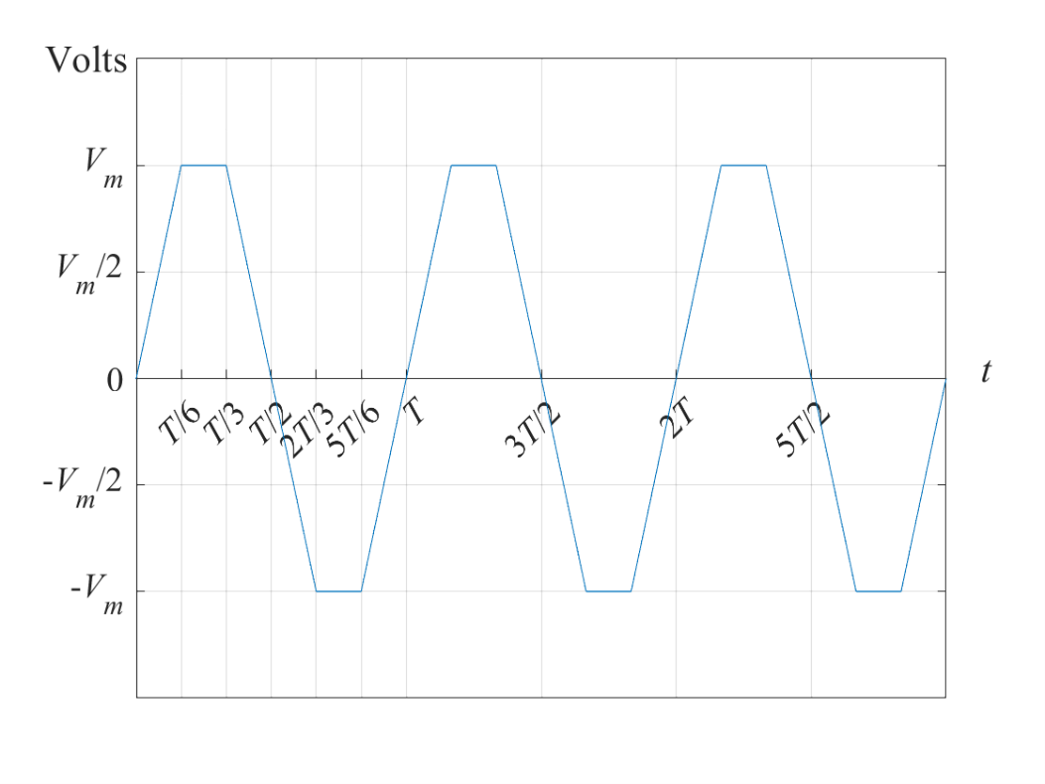
\includegraphics[width=1.0\textwidth]{questionbank/circuit_quantities/rms_trapeziod/v0/waveform.png}
\end{center}

% =========================================================
\begin{partquestion}{findrms}
{Find the root-mean-square (rms) voltage of the trapezoidal waveform.}
\begin{answer}

We start with the calculation for the average power dissipated in an arbitrary resistor $R$.

\[
P_{\text{avg}}
=
\frac{1}{T}\int_{0}^{T}p(t)\,dt
=
\frac{1}{RT}\int_{0}^{T}v^2(t)\,dt
\]

Since the trapezoidal waveform is piecewise linear, it makes sense to break up the integral into five separate regions for easier analysis. We can write:

\begin{align*}
P_{\text{avg}}
&=
\frac{1}{RT}
\Biggl[
\int_{0}^{T/6}
\left(\frac{6V_mt}{T}\right)^2 \dd t
+
\int_{T/6}^{T/3}
V_m^2 \dd t
+
\int_{T/3}^{2T/3}
\left(\frac{6V_m(T/2-t)}{T}\right)^2 \dd t
\\
&\qquad
+
\int_{2T/3}^{5T/6}
(-V_m)^2 \dd t
+
\int_{5T/6}^{T}
\left(\frac{6V_m(t-T)}{T}\right)^2 \dd t
\Biggr].
\end{align*}

Calculating the integrals leads to

\[
P_{\text{avg}}
=
\frac{1}{RT}
\left[
\left.\frac{12V_m^2}{T^2}t^3\right|_0^{T/6}
+
\left.V_m^2t\right|_{T/6}^{T/3}
+
\left.\frac{12V_m^2}{T^2}\left(t-\frac{T}{2}\right)^3\right|_{T/3}^{2T/3}
+
\left.V_m^2t\right|_{2T/3}^{5T/6}
+
\left.\frac{12V_m^2}{T^2}(t-T)^3\right|_{5T/6}^{T}
\right]
\]

which simplifies to

\[
\frac{5V_m^2}{9R}
=
\frac{V_{\text{rms}}^2}{R},
\]

so it follows that

\[
V_{\text{rms, trap}}
=
\frac{\sqrt{5}}{3}V_m.
\]

\end{answer}
\end{partquestion}

% =========================================================
\begin{partquestion}{ratio}
{What is the ratio of this rms voltage to that of a pure sinusoidal AC source with the same amplitude $V_m$ and period $T$?}
\begin{answer}

\[
\frac{V_{\text{rms, trap}}}{V_{\text{rms, sine}}}
=
\frac{\frac{\sqrt5}{3}V_m}
{\frac{1}{\sqrt2}V_m}
=
\frac{\sqrt{10}}{3}.
\]

\end{answer}
\end{partquestion}

% =========================================================
\begin{partquestion}{wavespecs}
{If $V_m=\qty{17}{\volt}$ and $T=\qty{17}{\milli\second}$, find the amplitude, the peak-to-peak voltage, the frequency, and the radial frequency of the trapezoidal waveform.}
\begin{answer}

The amplitude is simply

\[
V_m=\qty{17}{\volt}.
\]

The peak-to-peak voltage is

\[
V_{\text{pp}}
=
2V_m
=
2\left(\qty{17}{\volt}\right)
=
\qty{34}{\volt}.
\]

The frequency is

\[
f
=
\frac{1}{T}
=
\frac{1}{\qty{17}{\milli\second}}
=
\qty{58.8}{\hertz}.
\]

The radial frequency is

\[
\omega
=
2\pi f
=
2\pi(58.8)
=
\qty{369.6}{\radian\per\second}.
\]

\end{answer}
\end{partquestion}

\end{mainquestion}